\chapter{INTRODUCTION}
\label{chap-one}

\section{Background}

\subsection{History of Friction Science}
Research of friction, wear, and dissipation phenomena is collectively known as Tribology. From the Greek \textit{tr\'ib\={o}}, meaning 'to rub', the term 'tribology. came into wide usage following publication of The Jost Report in 1966\cite{101}. Despite that relatively recent terminology, human beings have been working with friction for some two-hundred-thousand years. Neanderthals shearing flakes from stone to form hunting tools, for example, will be discussed in some detail in Chapter 9. 

The first documented instance of the intentional use of lubricants dates to the fourth millennium B.C. Records suggest that both the Egyptians and Sumerians employed lubricants. Towards reducing the labor necessary for construction of the pyramids, the Egyptians spread water over sand to reduce the kinetic coefficient of friction between the ground and massive stone blocks \cite{104}. Sumerians began using grease for lubricating axles in the second millennium B.C.

Though there were these heuristic explorations of friction modifiers throughout ancient history, the first known, rigorous pursuit of friction science began with Leonardo Da Vinci (1452 - 1519). His notebooks, covering so many aspects of art and science, also include diagrams of blocks attached to rope being slid over surfaces. Involved in design, engineering, and construction for much of his patronage, overcoming the friction of sliding surfaces would have been of great interest to Da Vinci. Galileo Galilei (1564 - 1642) and Guillarme Amontons (1663 - 1705) also did critical work in establishing the early empirical rules of tribology. Some decades later, Charles Augustin-Coulomb (1736 - 1806) of electro-statics fame, would supply the third law of macro-scale friction behaviors. Until the 20th century, the following three friction laws represented the bulk of friction science. Amontons' published his friction work in 1699 while Coulomb contributed the third law in 1785, so they are all conventionally lumped together as "Amontons' Law".

\begin{enumerate}
\item The force of friction is proportional to the normal load.
\begin{equation}
\mathit{f} = \mu F_{n}
\label{ch1-eq:one}
\end{equation} 
\item The force of friction is independent of the apparent contact area.
\item The force of friction is independent of the sliding velocity.
\end{enumerate}

These three laws laid the foundation for advances in mechanical engineering and the design of industrial and agricultural implements. Still useful in macro-scale environments or when ignoring higher-order effects is permissible, the three classical laws of friction have been either supplanted or modified by modern tribological study. These important advances will be discussed in the next section, Modern Tribology.

\subsection{Modern Tribology}

The modern era of nanotribological study has been facilitated by the radical advancements in theoretical physics and mechanical instrumentation of the late 19th and 20th centuries. Precision mechanical instruments, often developed in the booming petroleum and chemical industries of the era, made possible the first investigations of near-atomic scale friction mechanisms. Atomic-scale adhesion and stick-slip behavior, topics often addressed in the Krim Nanotribology group, were introduced by G.A. Tomlinson and L. Prandtl in 1929 \cite{105}. In the middle portion of the 20th century, Bowden and Tabor showed that the force of friction is proportional to the true area of contact at the interface \cite{103}, a critical update to the second of Amontons' laws. Archard and Hirst demonstrated wear of un-lubricated, metal contacts and how the presence and deformation of asperities (the very small ridges and valleys on the surface of materials) contributed to frictional behavior. This group of scientists, though not the only contributors, established the foundation of modern Tribology in the first half of the 20th century.

For the field of tribology broadly, and for my work specifically, two developments from the last quarter of the 20th century take precedence.  With important results in 1986\cite{102} and 1988\cite{204}, the Quartz Crystal Micro-balance (QCM) was being employed for studies in interface friction and dissipation by Jacqueline Krim and colleagues at Northeastern University. The another notable advancement was the Atomic Force Microscope (AFM), developed as an extension of the Scanning Tunneling Microscope (STM) platform by Gerd Binnig's team, at IBM's Zürich, Switzerland facility in 1986 [citation needed]. Those two leaps forward in technology, combined with other well-established instruments including the Macro-scale Tribo-meter (MTM) and Scanning Electron Microscope (SEM) devices provide the greater part of the platform necessary for the work and results presented in this thesis. 

%Amontons' Laws, having carried science and engineering so far, saw improvement through the aforementioned era. At  updated as follows.
%
%\begin{enumerate}
%1) old = the force of friction is directly proportional to the normal load
%new = the force of friction is proportional to the true contact area, which is a non-linear function of the normal load, or something
%
%2) old = the force of friction is independent of the contact area
%new = the force of friction is proportional to the true contact area, which is not a contradiction, but perhaps 1 and 2 from the old era should be combined and replaced
%
%
%3) old = the force of friction is independent of the sliding velocity
%new = Mak, Krim, 1998, Phys Rev. B "QCM Studies of the velocity dependence of interfaciail friction" --> F ~ v<raised to the>n where n <1 for "low" values of v
%\end{enumerate}


\section{Project Motivations}

Explored in this thesis are selected topics primarily utilizing the Quartz Crystal Micro-balance to access nanometer-scale properties of solids, liquids \cite{106}, and gases at its interface. Several other instruments and techniques are involved but the QCM is the device which binds the works together. The topics explored include: (1) The impact of surface functional groups, and thus the electric charge, on the nanotribological properties of nanodiamonds (ND); (2) The nanotribological gaseous diffusion properties of water and ethanol in nano-pores with and without affixed membranes of hydrogenated, ie functionalized, graphene; (3) The adsorption of water and ethanol onto, and whether there is permeation through, hydrogenated graphene oxide flake-layers.

The remainder of this first chapter will be devoted to providing the motivation for each of these studies followed by a brief description of the necessary physics knowledge applied =in order to interpret the behavior of these systems as recorded.

\subsection{Societal Need}

According to Herodotus, a Greek historian who lived in the fifth century B.C., asphalt was used in Babylonian construction. The first use of petroleum for fuel occurred in the fourth century BCE \cite{107}. Despite this long history, the careful use of lubricants would have to wait until the technological field-day of the industrial revolution. Modern petroleum extraction techniques of the late 19th century, the wide adoption of the internal combustion engine in the early 20th century, and the massive growth of the chemical industries in the early and mid-20th century ushered in the lubricant-maintained technological world of today. 

Oil-sands were first mined in Merkwiller-Pechelbronn, Alsace, France (1745), under the direction of Louis Pierre Ancillon de la Sablonnière [citation needed!]. Despite the first modern petroleum refinery being built at that same site in 1857, petroleum-derivatives would not be widely accessed or used for more than a century. Two years later, in 1859, workers on an oil-rig in Titusville, Pennsylvania, USA, found that a parafin-like build-up, though annoying to remove from equipment, was useful as a salve and personal ointment. By 1870, Vaseline, a product refined by Robert Chesebrough from this raw material was in production at a factory in Brooklyn, NY, by a chemist named Robert Chesebrough [citation needed!].


This distillation of a topical salve and lubricant, from a raw petroleum product, was hardly the first instance in history where human beings had changed their friction environment. Nonetheless, it marks a moment where the fine-tuned refining of distillates, from petroleum, would become an omni-present factor in human development. Unfortunately, like with the invention of so many tools, with novel value comes novel danger. Though the materials were often noxious to the senses, an evolutionarily programmed warning for all living creatures, these industrial products were so immediately effective and important that it would take decades and several high profile disasters for unbridled thirst for oil and its products to be choked.

The most important moment in the history of environmental activism, for the United States, was Love Canal. In 1942, the Niagara Power and Development Company gave permission to Hooker Chemical Company to begin dumping toxic wastes into an abandoned canal in Western New York state. Excavated in the 1890's by William T. Love, the canal was intended to connect the sections of the Niagara River above and below the famed Niagara Falls to provide for a planned industrial, commercial, and residential community. Despite his vision for a Utopian residential-industrial community, his name would unfairly come to be associated with the site of the worst toxic contamination event in American History - the poisoning of families in Love Canal, Niagara Falls, New York.

Between 1942 and 1952, 21,800 tons of chemicals including caustics, alkalines, fatty acids, and chlorinated hydrocarbons were deposited into the clay-lined, dry canal. After capping the resevoir with clay, wastes contained in 55-gal metal or fiber barrels lay at most 25 feet below the ground. In short order, vegetation grew over the ground and the land was considered by Niagara Falls city officials for use in construction of either schools or homes for the booming city. In 1953, Hooker handed the deed to the land over to the City of Niagara Falls for 1 dollar and a liability limitation clause intended to shield the organization from any future lawsuits.

In the winter of 1977, a particularly heavy snow storm dumped between three and four feet of snow and over the course of weeks significantly raised the local water table. As that snow melted, it pushed a release of toxins from the buried waste repository into the backyards and basements of residents of Love Canal. Seeking aid from government officials, the land and water were tested for various aforementioned chemical wastes. Within weeks, the neighborhood was evacuated and sealed to all but a small handful of families who insisted on staying, though at the edges of the neighborhood. Love Canal would become the first federal Super Fund site and the clean-up and reports would provide painful support for an expanded and strengthed Environmental Protection Agency (EPA), founded by Richard Millhouse Nixon. 

The insatiable appetite for chemical products, including lubricants, with unlimited upside and only unknown dangers had incurred a tragic toll. The search for non-toxic, environment and human-friendly lubricants, though nascent at that moment, has only ever increased.

Many pathways to improvement of lubrication with a simultaneous decrease in the toxicity and danger of them are being pursued. Figure 1 gives detail regarding the families of materials employed as the cutting-edge of lubrication as a function of time.

\begin{figure}[hbtp]
	\centering
	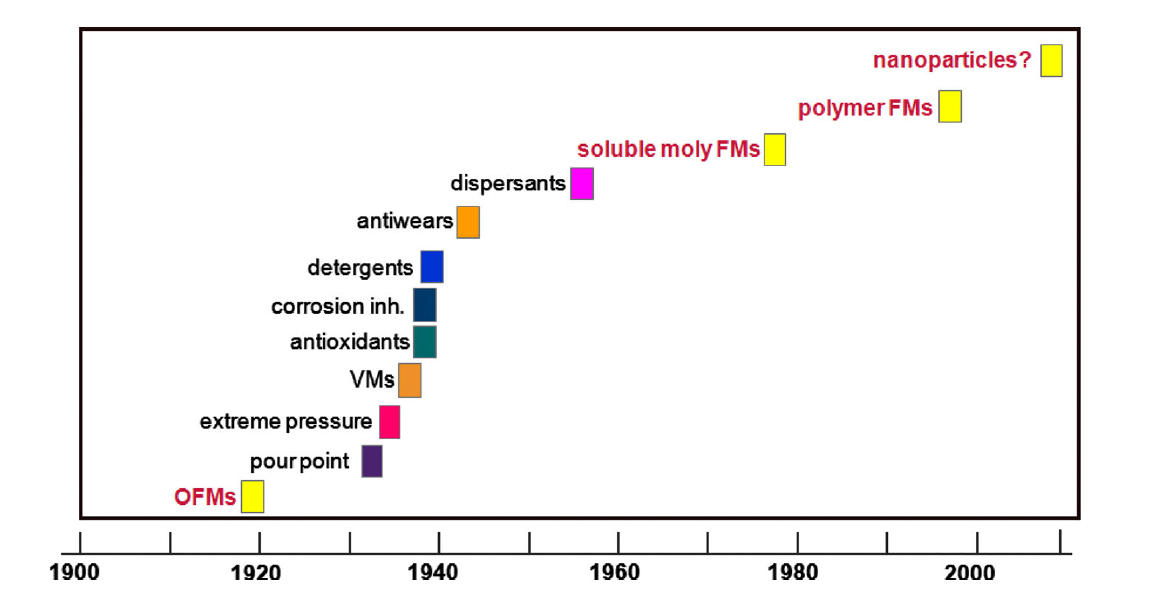
\includegraphics[width=1.0\textwidth]{Chapter-1/fig1_spikes_timeline}
	\caption{Overview of lubricant additives and friction modifiers. Borrowed from Spikes, 2015}
	\label{fig1-spikes-timeline}
\end{figure}


The impetus to change directions from hydrocarbon-based to nanoparticle-based lubricants is not only pushed by the desire to improve human, animal, and environmental health but also pulled by the promise of more effective and efficient lubrication and wear-reduction systems. The impacts of tribology are ubiquitous. Whether discussing economics, the environment, industrial maintenance, changing a car's engine oil, or ice skating,  friction, dissipation, and wear are always issues to be considered. Since the publication of The Jost Report in 1966, interest in and funding for tribological research has accelerated \cite{101}. An oft cited, and important touchstone for the practical importance of tribology, is that a an internal combustion engine utilizing diesel fuel will use 10 \% of the energy from that fuel to overcome internal frictional losses[ZL ref 2,3]. A lowering of those losses to 9 \% is estimated to potentially save one billion gallons of diesel fuel, per year, in the United States. Beyond the fuel expense and diesel exhaust savings, that reduction in frictional dissipation also translates to less wear and tear on the individual engines and thus a potential decrease in maintenance downtime for owners and operators. From this single example, it becomes clear the sort of impacts which tribology is capable of making across the spectrum of the economic and environmental landscapes.


\subsection{Topic 1: Comparison Study of Nanodiamonds Having Positively or Negatively Charged Surface Functional Groups and their Impact on Tribological Behavior}

\subsubsection{Topic 1 Hypothesis}

Following work done by Zijian Liu [cite RSC Adv paper], the predominant hypothesis was that the surface conductivity of a QCM sample would determine which (and whether) a nanodiamond having a particular surface charge, as a function of its surface chemical groups, would experience tribological interactions. It was supposed that an insulating material (Al2O3) and contacting nanodiamond solution would not exhibit significant attraction whereas a conducting material (stainless steel) would exhibit significant attraction, as understood by surface image charge effects.


\subsubsection{Topic 1 Background}

Though the petroleum and synthetic chemical industries have made profound improvements to lubrication in the 20th and early 21st centuries, the secondary effects of these lubricants[insert ref, harmful effects of lubricants] provide strong reason to find novel, less toxic, and more durable lubricants and lubricant additives for both industry, research, and household use. Nanometer-scale particles of many species are emerging as effective lubricant additives [insert ref], much of the work done in oil-based media. Studies of nanodiamonds have shown their ability to lubricate for a long duration with degradation, a common problem for lubricants, though minimal work has been done to examine the lubricant behavior of nanodiamonds in aqueous solution. Further, the importance of surface chemical groups for tribology has been investigated [insert ref]. Here we report the first analysis of the importance to tribology of variation of surface functional groups on nanodiamonds. Carboxylated nanodiamonds were shown to be an effective lubricant for both alumina-on-alumina interfaces as well as stainless-steel-on-stainless-steel interfaces, as tested in a ball-on-disc MTM. On the other hand, hydroxylated nanodiamonds were shown to be either ineffectual in changing the tribology at the interface, for alumina MTM contacts, or to be anti-lubricating, producing an increase in the coefficient of kinetic friction for stainless steel MTM contacts.


\subsection{Topic 2 - The Impact of Root-mean-square (RMS) Surface Roughness on Nanotribological Behaviors for Gold Surfaces}


\subsubsection{Topic 2 Hypothesis}

The study of smooth versus rough gold was conducted following from the hypothesis that a dramatic difference in orders of magnitude difference in the RMS surface roughness of two otherwise identical substrates would have a defining impact on how a set of nanoparticles would interact with those substrates. 

It was proposed that surface geometry at the nanoscale must be known to understand macroscale friction effects.  Nanodiamonds of diameter ~5 nm have a known friction reduction effect (REF 1 - Ozawa, 2007; REF 2 - Liu, 2015,). This effect is thought to be due to polishing of the solution-contacting interface. If the primary action of the nanodiamonds is to polish, there are two possible pathways. It may be that there is a removal of jutting-out asperities OR that there is a filling-in of voids between asperities. The following methods will explore what is occurring at the important scale.

The expectation  at the outset was that a much rougher surface would exhibit a much greater degree of polishing when exposed to a hard particle such as a nanodiamond. If polishing occurs, and the hypothesis is true, this effect ought to be displayed dramatically by gold surfaces having orders-of-magnitude difference in RMS surface rougness between them, as our samples do.



\subsubsection{Topic 2 Background}

This study explores the nanoscale and macroscale tribological attributes of alumina and stainless steel surfaces immersed in aqueous suspensions of positively (hydroxylated) or negatively (carboxylated) charged nanodiamonds (ND). Following on previous work by Dr. Zijian Liu, a Krim group alumnus, this study explores the connection between microscopic (QCM and AFM) effects which result from exposure of metallic and ceramic surfaces to aqueous nanodiamond solutions with the macro-scale lubrication behavior of these same combinations of surfaces and solutions.


\subsection{Topic 3 - The Tribological Behavior of Super-paramagnetic Nanoparticles in Solution at the Interface With and Without the Presence of an External Magnetic Field}


\subsubsection{Topic 3 Hypothesis}

This study explored whether an external, applied magnetic field can influence friction and wear dynamics, at an interface, in the presence of superparamagnetic iron (III) oxide nanoparticles. Such particles have been demonstrated to greatly reduce the volume of material wear when the diameter of the particles was small enough (~30 nm). This reduction in wear is attributed to tribo-sintering of the nanoparticles into a tribo-film on the contacting surfaces (REF 3 and 5  - Kato, 2003, 2008; REF 4 – Kato and Komai, 2006). The production of such a tribo-film is dependent upon the oxygen diffusivity rate of the oxide nanoparticle introduced. High diffusivity among certain oxide species, such as Fe2O3 and Bi2O3, demonstrates a greater ability to produce a tribo-film and in turn dramatically reduce wear volume. This study asks the question: what level of  influence does an external magnetic field exhibit on tribo-film formation, friction, and wear at an interface containing ferrimagnetic nanoparticles, which are otherwise known to lubricate?


\subsubsection{Topic 3 Background}

Certain nanoparticles, gamma-type iron oxide of nominal diameter of 5 nanometers, in this study, exhibit superparamagnetism. Superparamagnetism is the character of a particle such that its entire structure constitutes a single magnetic domain. Thus, as the magnetic moment of the particle respods to an external, applied magnetic field, so does the physical geometry of that particle in terms of its position and orientation. [citations needed]

Previous studies in the NCSU nano-tribology group, conducted by Dr. Zachary Fredricks, explored the paramagnetic behavior of oxygen molecules, at low temperature, in vacuum, on a metallic surface. Through the application and removal of an external magnetic field, the rotational and spatial orientation of these molecules was seen to change, producing an effect in the dissipation as measured by the QCM. [zach thesis citations needed]

The study of superparamagnetic, aqueous iron oxide nanoparticles explores if and how such behaviors manifest in a aqueous, room temperature rather than evacuated, low temperature environment.


\subsection{Topic 4 - Permeation of Gaseous Water and Ethanol into or through Hydrogenated Graphene and Hydrogenated Graphene Oxide}

\subsubsection{Topic 4 Background}
Filtration and Purification, as well as gas separation and retention [ref about helium shortage needed] are practical drivers behind the growing interest in graphene and modified graphene membranes. The study of graphene as a membrane gained particular notoriety upon the observation that a helium-leak-tight graphene membrane is permeable to water\cite{108}. Not only permeable, graphene exhibited extremely low frictional interactions to the diffusion of water through its structure. This work built upon previous work conducted in the Krim Group by Zijian Liu. Whereas his studies utilized graphene membrane layers on top of flat aluminum substrates, the experiments discussed here transition the studies to hydrogenated graphene layers atop nano-porous aluminum oxide substrates. These nano-porous structures, having greater than a billion pores  on the surface of the QCM, increase the working surface area underneath the graphene layers by a factor greater than 100. This great leap in surface area for adsorption of gases which have permeated through the hydrogenated graphene membrane, provide an improvement in sensitivity and reduction of uncertainty in measurements. The porous alumina samples, grown by Dr. Antonin Marek in the NCSU Department of Chemistry, as part of our collaboration with the Smirnov group, follow from well-established methods for anodizing aluminum\cite{109}.

These studies, introducing ethanol and water vapor, separately and during different trials, to the hydrogenated graphene membranes, investigate whether such membranes impede or admit either gas species or if instead the gas species physically or chemically alter said membranes. This work also builds upon work done by Zijian Liu in pursuit of his doctoral degree.

Previous studies, including work done by Nair et al \cite{108}, report the behavior of graphene oxide layers including the impermeability to helium and ethanol. On the other hand, it has been shown that water will flow through a graphene oxide flake layer structure with very low friction. Efforts by Zijian Liu and myself in recording gaseous adsorption isotherms of either water or ethanol demonstrate the behavior of a hydrogenated graphene oxide layer structure in terms of permeability or impediment to flow.

\subsubsection{Topic 4 Hypothesis}


The studies of hydrogenated graphene oxide and hydrogenated graphene layers, on porous alumina substrates, and the exposure of these membranes to either water vapor or ethanol, in vacuum, were conducted following work done in Krim Nanotribology lab[cite Zijian thesis, others], as well as elsewhere in the tribology community[cite Nair et al, others], which demonstrated the impermeability or permeability of graphene and graphene-oxide type membranes to various gaseous species.

Due to the hydrogenation of these two membrane types, graphene and graphene oxide layers, the hydrophobicity of each material was increased [cite C]. The water vapor permeability of each membrane was thus expected to decrease without substantial change in the permeability to ethanol vapor, a non-polar molecule. Comparison with work done by Zijian Liu utilizing un-hydrogenated graphene and graphene oxide layers  is reported.

\addcontentsline{toc}{section}{{Chapter 1 References}}
